The GDELT data subset we use in this project consists of sixty
three thousand csv files, where each file takes somewhere between
800 KB and 1.5 MB of storage.

On our P2 hand-in we include a script
(/gdelt/download.py) that downloads each csv file
and edits the filenames for further processing.
If a file is found to be corrupt, it is not downloaded and
the index of the file is saved in a .txt file
(/gdelt/bad\_indices.txt).

The dataset consists of sixty attributes and the domain of
each attribute is in detail on the official handbook
{\color{red}{citation}}.

Moving on, the suicide rate dataset can be obtained from
the Centers for Disease Control and Prevention
website \cite{suicide_website}.

The election results dataset is straightforward, it can be
obtained on {\color{red}{todo}}.

\begin{figure}
	\centering
	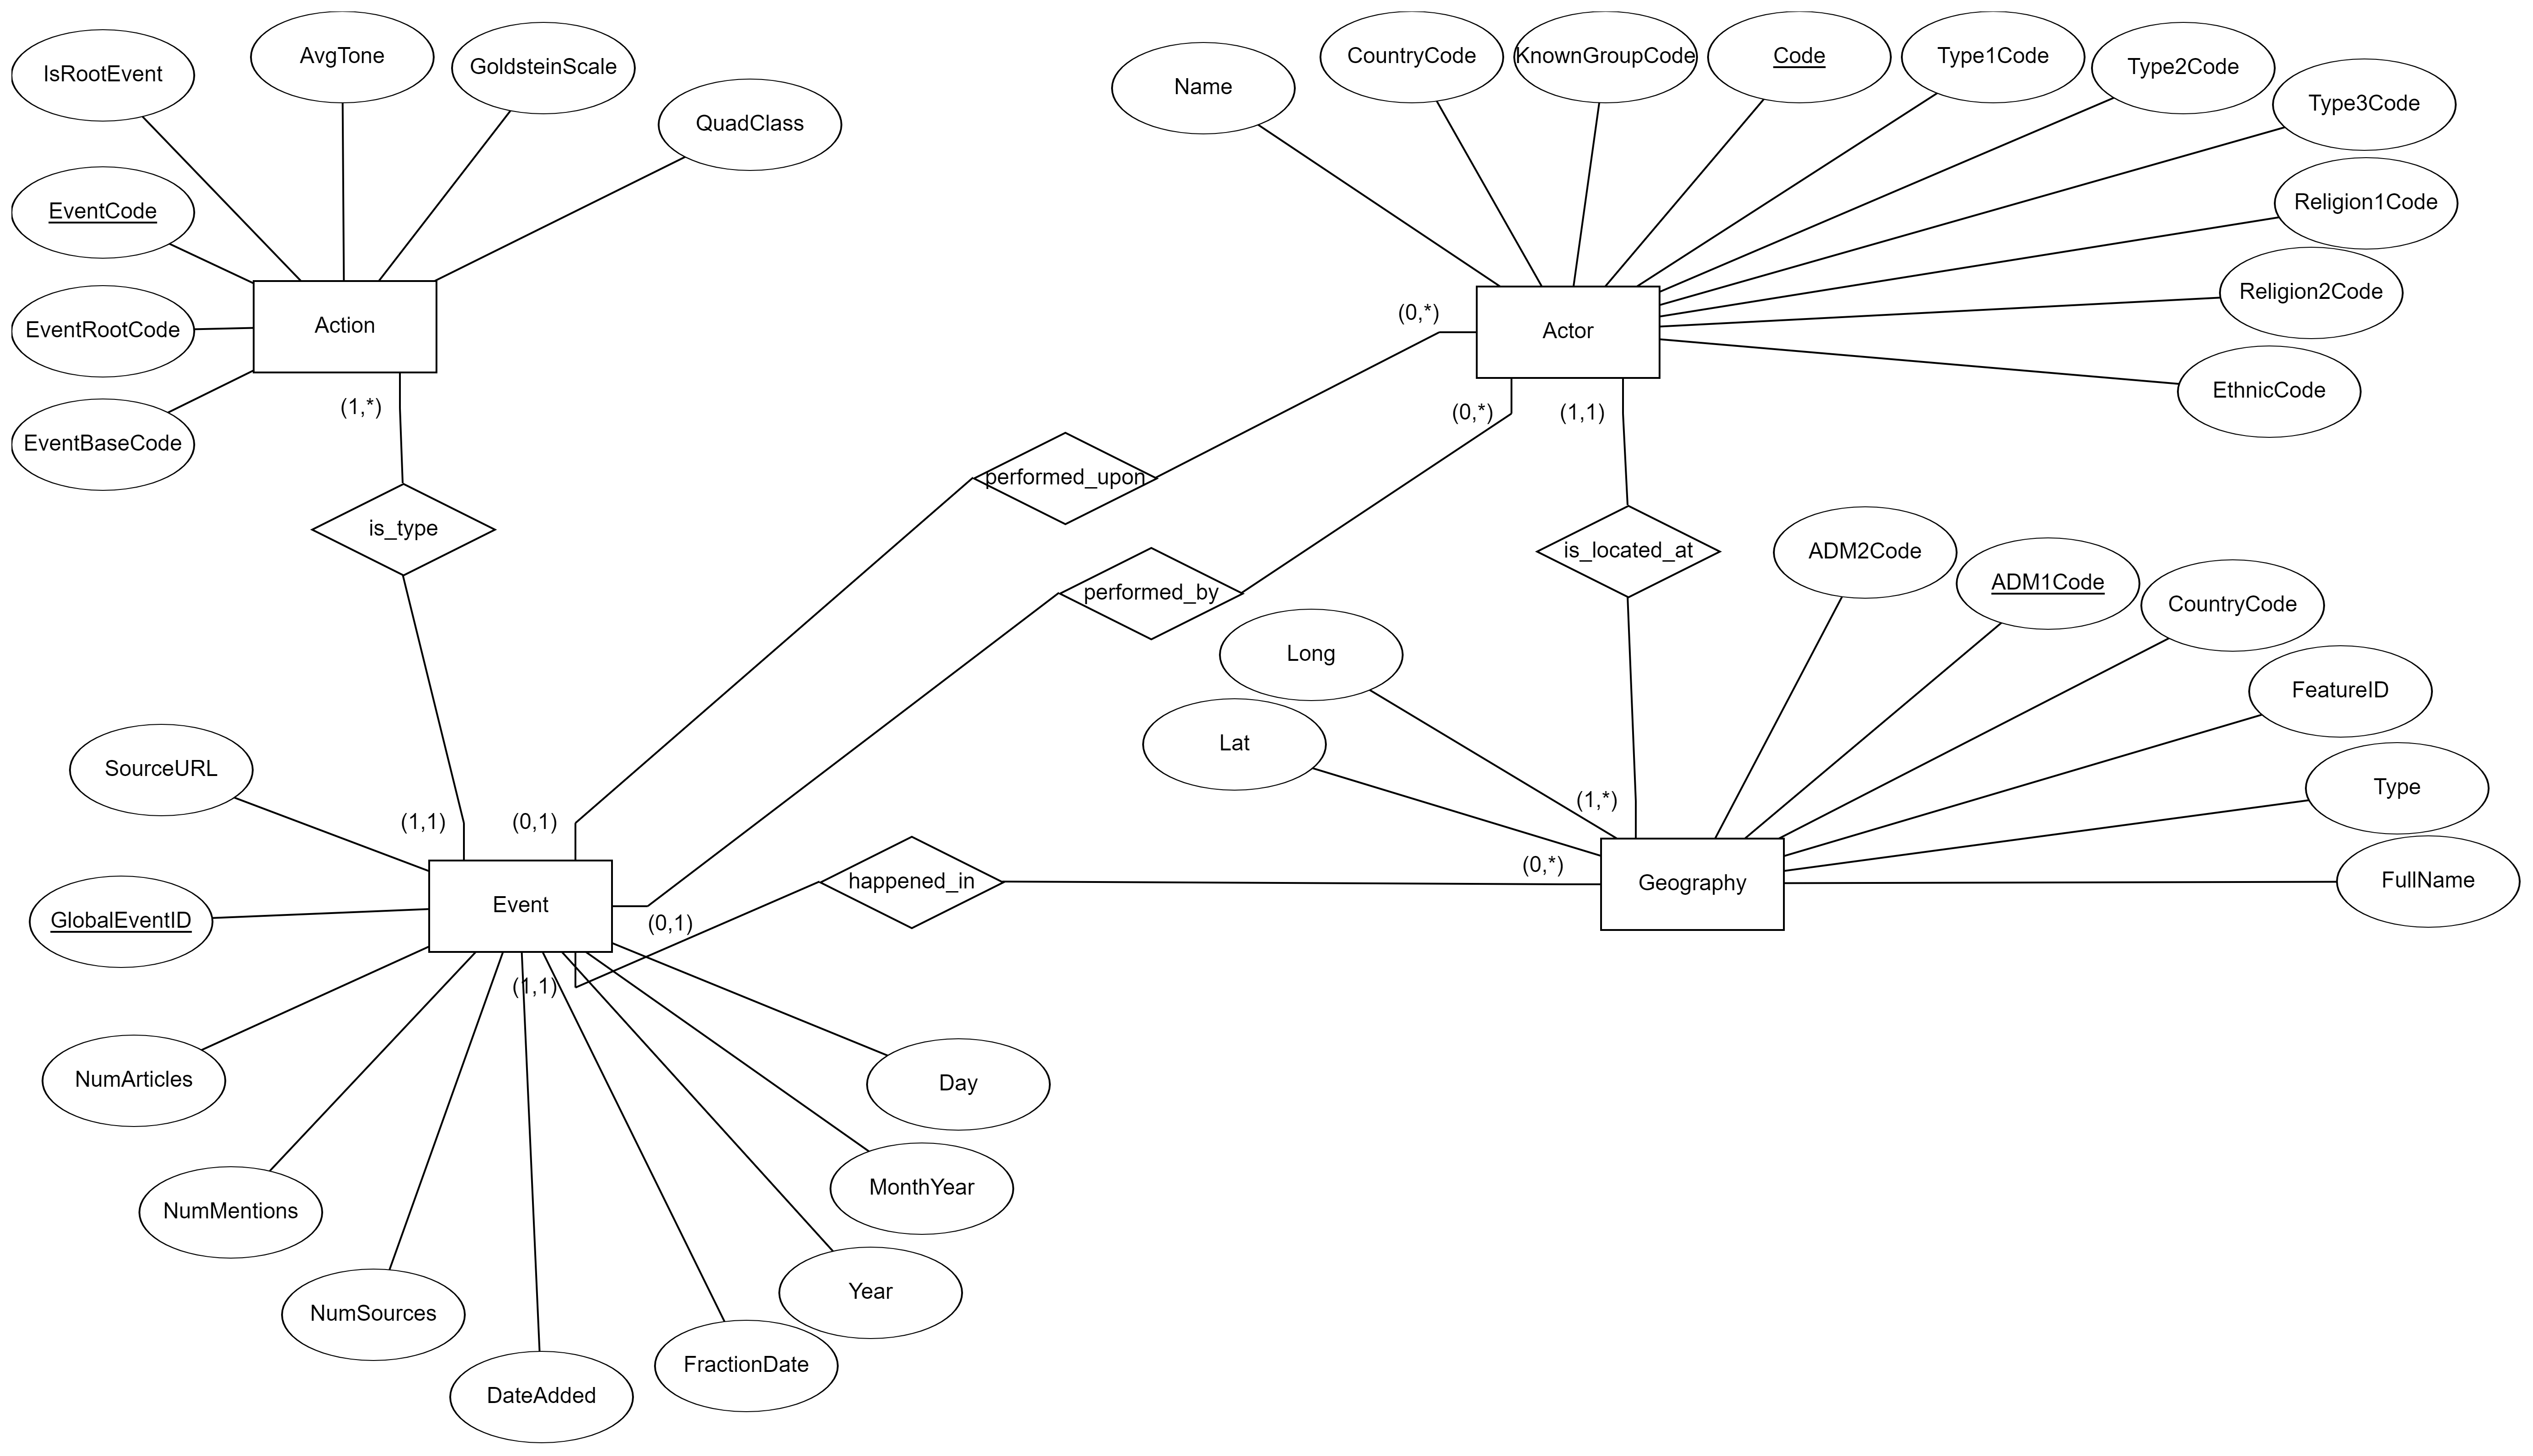
\includegraphics[scale = 0.08]{gdelt}
	\caption{Our GDELT schema integration}
	\label{fig:gdelt}
\end{figure}

\begin{figure}
	\centering
	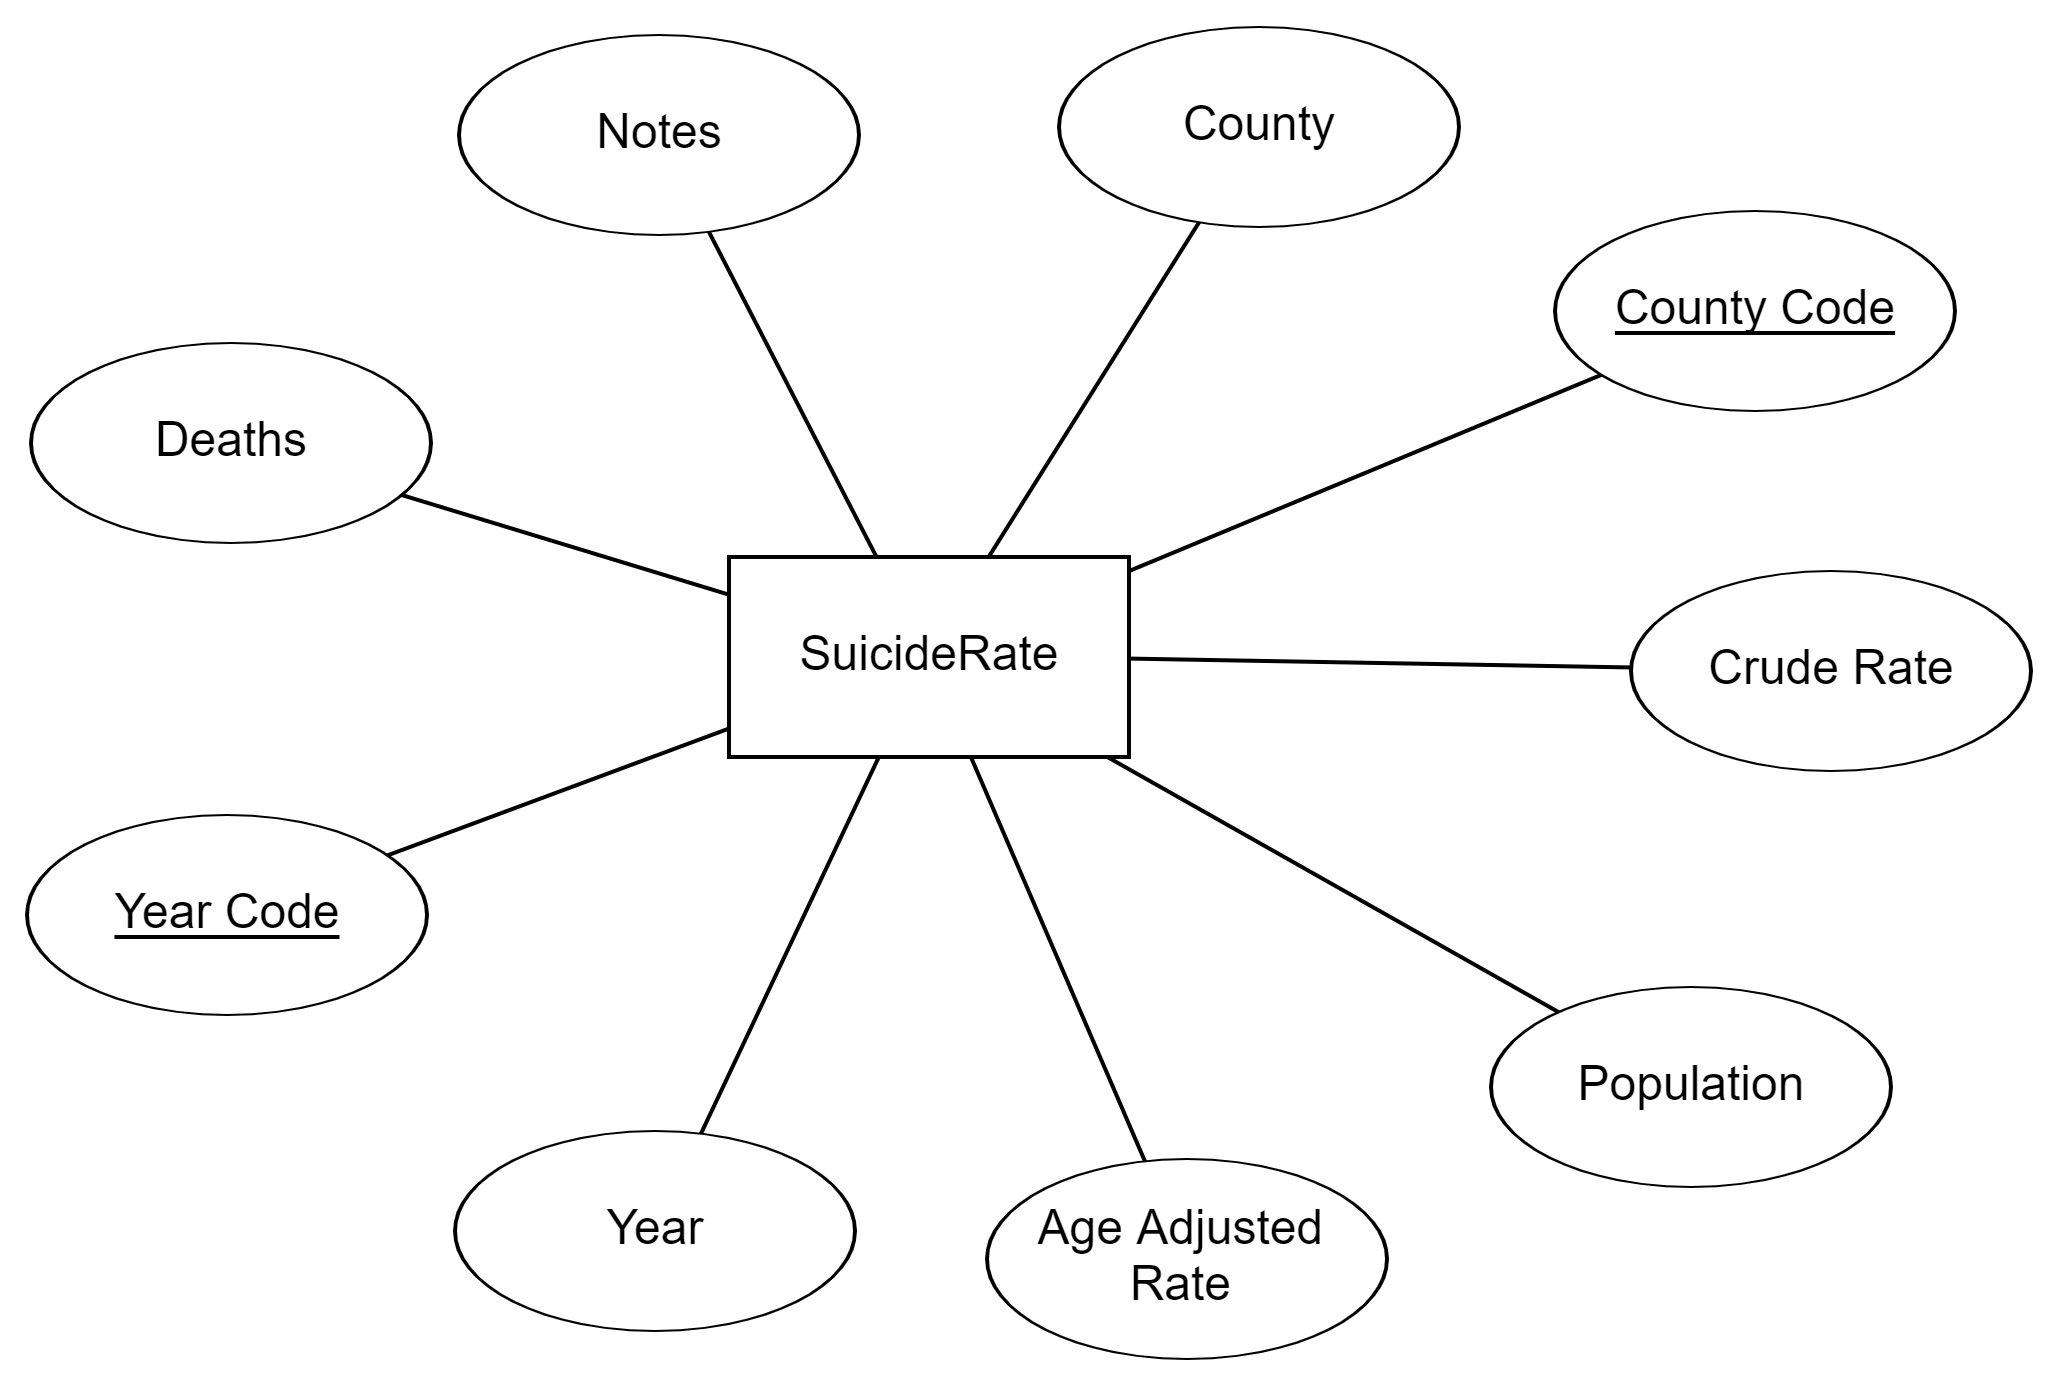
\includegraphics[scale = 0.18]{suicide_rate}
	\caption{Our suicide rate schema integration}
	\label{fig:suicide_rate}
\end{figure}

\begin{figure}
	\centering
	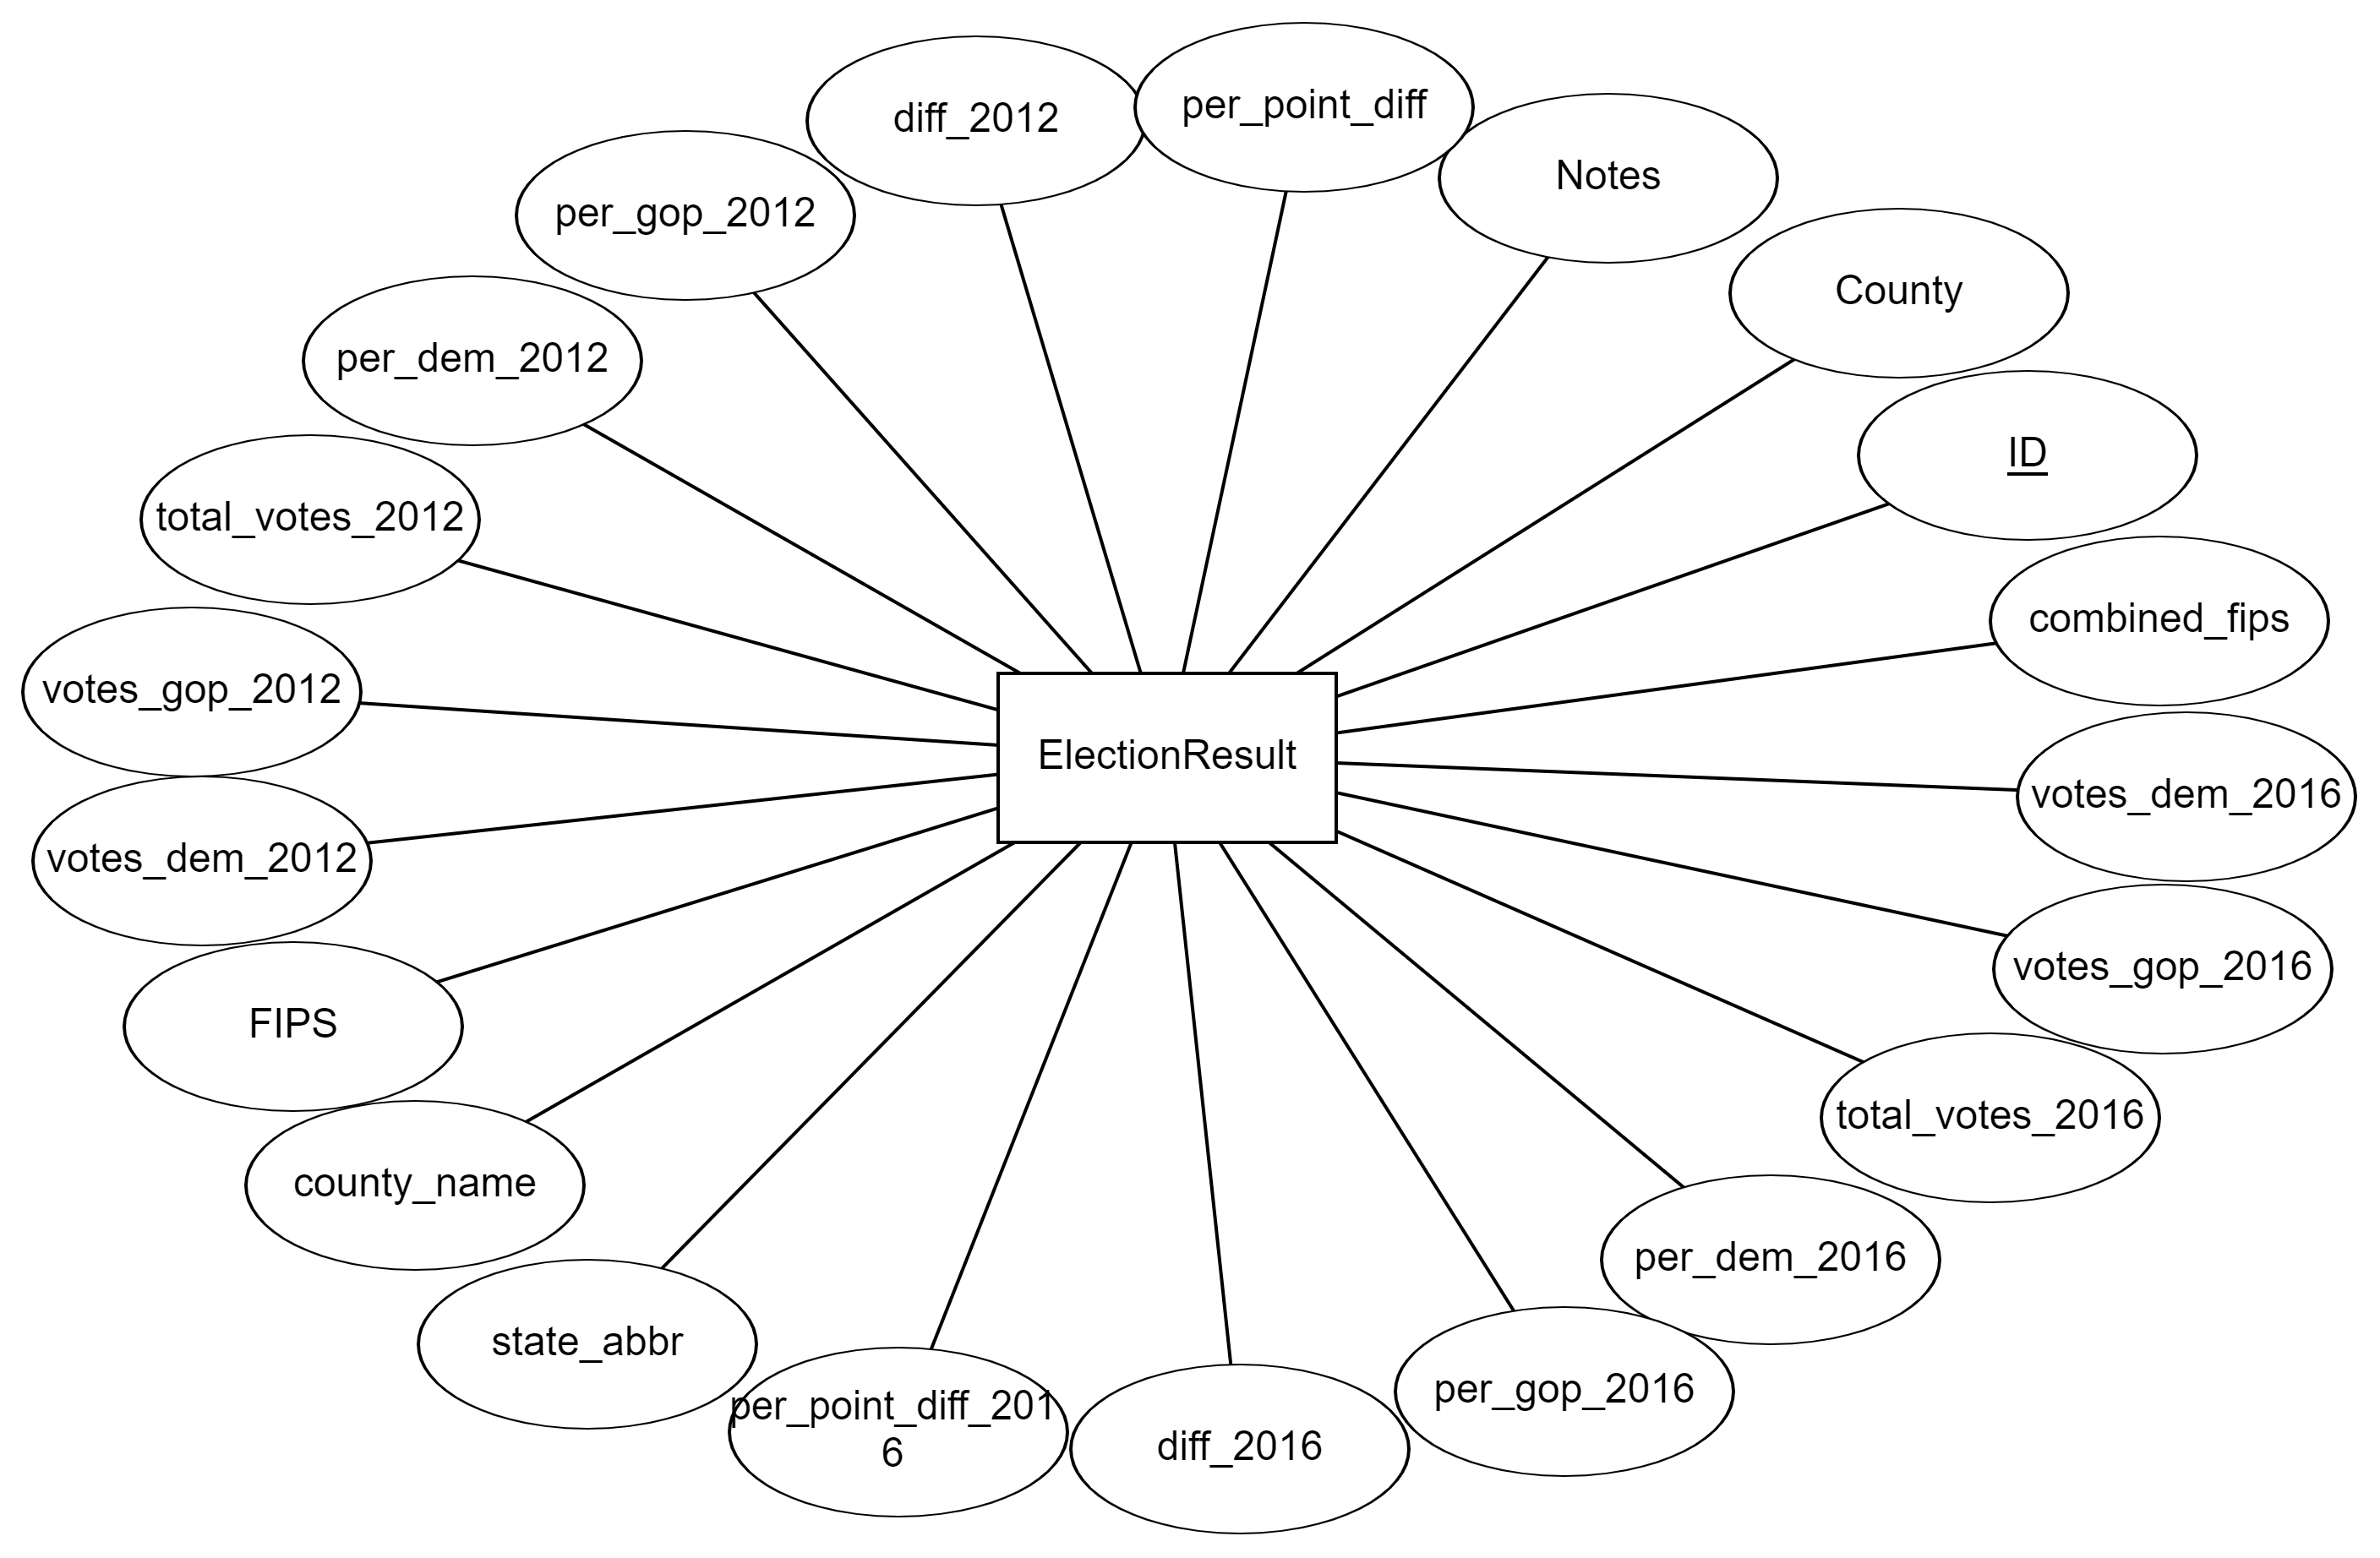
\includegraphics[scale = 0.12]{election_results}
	\caption{Our election results integration}
	\label{fig:election_results}
\end{figure}

\begin{figure}
	\centering
	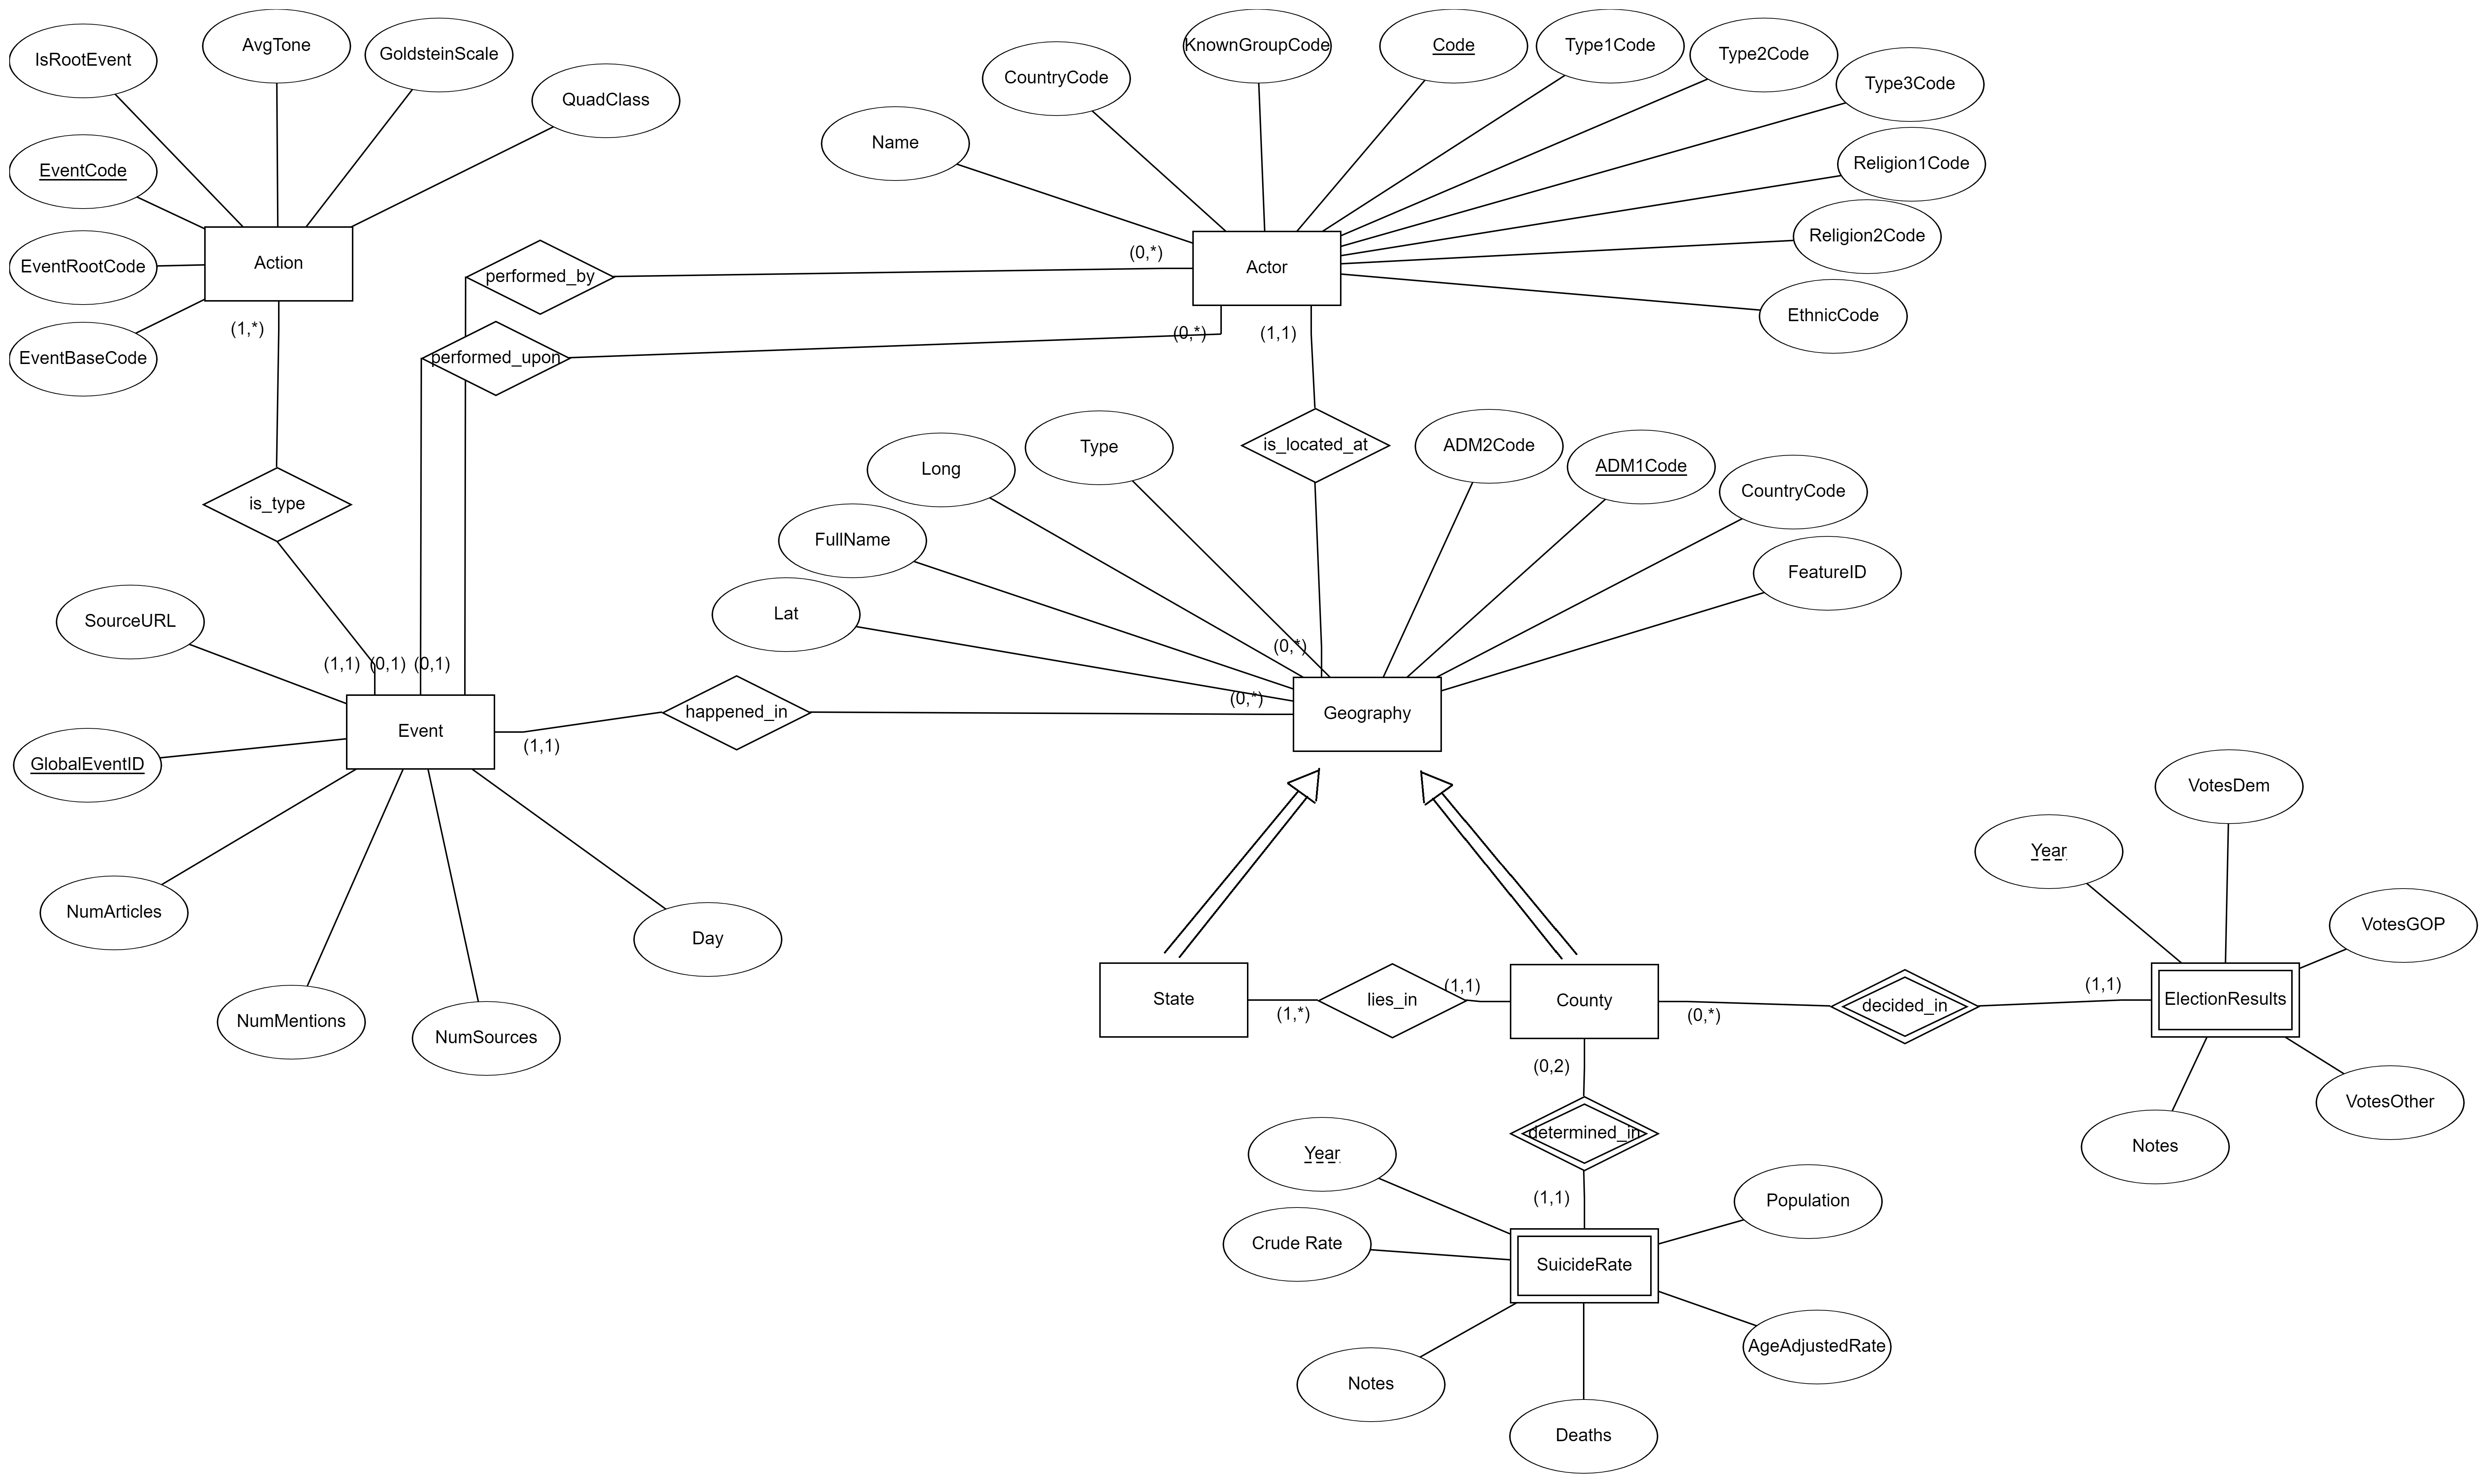
\includegraphics[scale = 0.08]{all}
	\caption{Schema over the whole database}
	\label{fig:all}
\end{figure}


\textbf{Putting it all together}:
The election results and the Suicide Rate data sets have the
county attribute in common.
A county lies in a state, and both a county and a state are
spesializations of a "geography".
Some other attributes can be removed since they are redundant
(e.g. MonthYear makes the Year attribute irrelevant).
The end result can be seen on figure \ref{fig:all}.

\textbf{Technical parts}
On the inegration process, we tried using the counties' FIPS codes
present on each of the datasets to link the different entities
together.
However we quickly learned that each dataset's FIPS code
contradicts the FIPS code each other data set.

Our solution has been to identify each county (and state)
by a geoID code than can be derived from {\color{red}{todo
https://community.esri.com/thread/24614
ESRI
}}.

The only other hazard occurs when ElectionResults generates an
ID that does not match any County, in that case the corresponding
row is simply skipped and also printed to STDOUT for reference.
